\documentclass[
  man,
  floatsintext,
  longtable,
  nolmodern,
  notxfonts,
  notimes,
  colorlinks=true,linkcolor=blue,citecolor=blue,urlcolor=blue]{apa7}

\usepackage{amsmath}
\usepackage{amssymb}




\RequirePackage{longtable}
\RequirePackage{threeparttablex}

\makeatletter
\renewcommand{\paragraph}{\@startsection{paragraph}{4}{\parindent}%
	{0\baselineskip \@plus 0.2ex \@minus 0.2ex}%
	{-.5em}%
	{\normalfont\normalsize\bfseries\typesectitle}}

\renewcommand{\subparagraph}[1]{\@startsection{subparagraph}{5}{0.5em}%
	{0\baselineskip \@plus 0.2ex \@minus 0.2ex}%
	{-\z@\relax}%
	{\normalfont\normalsize\bfseries\itshape\hspace{\parindent}{#1}\textit{\addperi}}{\relax}}
\makeatother




\usepackage{longtable, booktabs, multirow, multicol, colortbl, hhline, caption, array, float, xpatch}
\setcounter{topnumber}{2}
\setcounter{bottomnumber}{2}
\setcounter{totalnumber}{4}
\renewcommand{\topfraction}{0.85}
\renewcommand{\bottomfraction}{0.85}
\renewcommand{\textfraction}{0.15}
\renewcommand{\floatpagefraction}{0.7}

\usepackage{tcolorbox}
\tcbuselibrary{listings,theorems, breakable, skins}
\usepackage{fontawesome5}

\definecolor{quarto-callout-color}{HTML}{909090}
\definecolor{quarto-callout-note-color}{HTML}{0758E5}
\definecolor{quarto-callout-important-color}{HTML}{CC1914}
\definecolor{quarto-callout-warning-color}{HTML}{EB9113}
\definecolor{quarto-callout-tip-color}{HTML}{00A047}
\definecolor{quarto-callout-caution-color}{HTML}{FC5300}
\definecolor{quarto-callout-color-frame}{HTML}{ACACAC}
\definecolor{quarto-callout-note-color-frame}{HTML}{4582EC}
\definecolor{quarto-callout-important-color-frame}{HTML}{D9534F}
\definecolor{quarto-callout-warning-color-frame}{HTML}{F0AD4E}
\definecolor{quarto-callout-tip-color-frame}{HTML}{02B875}
\definecolor{quarto-callout-caution-color-frame}{HTML}{FD7E14}

%\newlength\Oldarrayrulewidth
%\newlength\Oldtabcolsep


\usepackage{hyperref}




\providecommand{\tightlist}{%
  \setlength{\itemsep}{0pt}\setlength{\parskip}{0pt}}
\usepackage{longtable,booktabs,array}
\usepackage{calc} % for calculating minipage widths
% Correct order of tables after \paragraph or \subparagraph
\usepackage{etoolbox}
\makeatletter
\patchcmd\longtable{\par}{\if@noskipsec\mbox{}\fi\par}{}{}
\makeatother
% Allow footnotes in longtable head/foot
\IfFileExists{footnotehyper.sty}{\usepackage{footnotehyper}}{\usepackage{footnote}}
\makesavenoteenv{longtable}

\usepackage{graphicx}
\makeatletter
\newsavebox\pandoc@box
\newcommand*\pandocbounded[1]{% scales image to fit in text height/width
  \sbox\pandoc@box{#1}%
  \Gscale@div\@tempa{\textheight}{\dimexpr\ht\pandoc@box+\dp\pandoc@box\relax}%
  \Gscale@div\@tempb{\linewidth}{\wd\pandoc@box}%
  \ifdim\@tempb\p@<\@tempa\p@\let\@tempa\@tempb\fi% select the smaller of both
  \ifdim\@tempa\p@<\p@\scalebox{\@tempa}{\usebox\pandoc@box}%
  \else\usebox{\pandoc@box}%
  \fi%
}
% Set default figure placement to htbp
\def\fps@figure{htbp}
\makeatother


% definitions for citeproc citations
\NewDocumentCommand\citeproctext{}{}
\NewDocumentCommand\citeproc{mm}{%
  \begingroup\def\citeproctext{#2}\cite{#1}\endgroup}
\makeatletter
 % allow citations to break across lines
 \let\@cite@ofmt\@firstofone
 % avoid brackets around text for \cite:
 \def\@biblabel#1{}
 \def\@cite#1#2{{#1\if@tempswa , #2\fi}}
\makeatother
\newlength{\cslhangindent}
\setlength{\cslhangindent}{1.5em}
\newlength{\csllabelwidth}
\setlength{\csllabelwidth}{3em}
\newenvironment{CSLReferences}[2] % #1 hanging-indent, #2 entry-spacing
 {\begin{list}{}{%
  \setlength{\itemindent}{0pt}
  \setlength{\leftmargin}{0pt}
  \setlength{\parsep}{0pt}
  % turn on hanging indent if param 1 is 1
  \ifodd #1
   \setlength{\leftmargin}{\cslhangindent}
   \setlength{\itemindent}{-1\cslhangindent}
  \fi
  % set entry spacing
  \setlength{\itemsep}{#2\baselineskip}}}
 {\end{list}}
\usepackage{calc}
\newcommand{\CSLBlock}[1]{\hfill\break\parbox[t]{\linewidth}{\strut\ignorespaces#1\strut}}
\newcommand{\CSLLeftMargin}[1]{\parbox[t]{\csllabelwidth}{\strut#1\strut}}
\newcommand{\CSLRightInline}[1]{\parbox[t]{\linewidth - \csllabelwidth}{\strut#1\strut}}
\newcommand{\CSLIndent}[1]{\hspace{\cslhangindent}#1}


\usepackage[nolongtablepatch]{lineno}
\linenumbers



\usepackage{newtx}

\defaultfontfeatures{Scale=MatchLowercase}
\defaultfontfeatures[\rmfamily]{Ligatures=TeX,Scale=1}





\title{eyetools: an R package for simplified analysis of eye data}


\shorttitle{eyetools: eye data analysis}


\usepackage{etoolbox}








\authorsnames{Tom Beesley,Matthew Ivory}





\affiliation{
{Lancaster University}}




\leftheader{Beesley and Ivory}



\abstract{Abstract goes here}

\keywords{eye-tracking; fixations; saccades; areas-of-interest}

\authornote{\par{\addORCIDlink{Tom Beesley}{0000-0003-2836-2743}} 

\par{       }
\par{Correspondence concerning this article should be addressed to Tom
Beesley, Lancaster University, Department of Psychology, Lancaster
University, UK, LA1 4YD, UK, Email: t.beesley@lancaster.ac.uk}
}

\makeatletter
\let\endoldlt\endlongtable
\def\endlongtable{
\hline
\endoldlt
}
\makeatother

\urlstyle{same}



\makeatletter
\@ifpackageloaded{caption}{}{\usepackage{caption}}
\AtBeginDocument{%
\ifdefined\contentsname
  \renewcommand*\contentsname{Table of contents}
\else
  \newcommand\contentsname{Table of contents}
\fi
\ifdefined\listfigurename
  \renewcommand*\listfigurename{List of Figures}
\else
  \newcommand\listfigurename{List of Figures}
\fi
\ifdefined\listtablename
  \renewcommand*\listtablename{List of Tables}
\else
  \newcommand\listtablename{List of Tables}
\fi
\ifdefined\figurename
  \renewcommand*\figurename{Figure}
\else
  \newcommand\figurename{Figure}
\fi
\ifdefined\tablename
  \renewcommand*\tablename{Table}
\else
  \newcommand\tablename{Table}
\fi
}
\@ifpackageloaded{float}{}{\usepackage{float}}
\floatstyle{ruled}
\@ifundefined{c@chapter}{\newfloat{codelisting}{h}{lop}}{\newfloat{codelisting}{h}{lop}[chapter]}
\floatname{codelisting}{Listing}
\newcommand*\listoflistings{\listof{codelisting}{List of Listings}}
\makeatother
\makeatletter
\makeatother
\makeatletter
\@ifpackageloaded{caption}{}{\usepackage{caption}}
\@ifpackageloaded{subcaption}{}{\usepackage{subcaption}}
\makeatother

% From https://tex.stackexchange.com/a/645996/211326
%%% apa7 doesn't want to add appendix section titles in the toc
%%% let's make it do it
\makeatletter
\xpatchcmd{\appendix}
  {\par}
  {\addcontentsline{toc}{section}{\@currentlabelname}\par}
  {}{}
\makeatother

%% Disable longtable counter
%% https://tex.stackexchange.com/a/248395/211326

\usepackage{etoolbox}

\makeatletter
\patchcmd{\LT@caption}
  {\bgroup}
  {\bgroup\global\LTpatch@captiontrue}
  {}{}
\patchcmd{\longtable}
  {\par}
  {\par\global\LTpatch@captionfalse}
  {}{}
\apptocmd{\endlongtable}
  {\ifLTpatch@caption\else\addtocounter{table}{-1}\fi}
  {}{}
\newif\ifLTpatch@caption
\makeatother

\begin{document}

\maketitle


\setcounter{secnumdepth}{-\maxdimen} % remove section numbering

\setlength\LTleft{0pt}

\resetlinenumber[1]

\section{Introduction}\label{introduction}

Eye tracking is a widely used technique in behavioural sciences, such as
attention, learning, and decision making
(\citeproc{ref-orquin2019primer}{Orquin \& Holmqvist, 2019}). By
recording the movement of an individual's gaze during research studies,
researchers can quantify where and how long individual's look at stimuli
presented on screen. Eye tracking offers an insight into real-time
cognitive processing, allowing researchers to infer mental states and
processes with high temporal precision
(\citeproc{ref-duchowski2017eye}{Duchowski \& Duchowski, 2017}). The
most common eye tracking systems use infrared light to detect
reflections from the eyes enabling the calculation of gaze position on a
screen. Once this data has been collected, it can be classified into
fixations and saccades. Fixations are time periods where the eyes remain
relatively stationary which enable focused attention on stimuli
(\citeproc{ref-rayner1998eye}{Rayner, 1998}). Conversely, saccades are
the rapid eye movements between fixations that are typically too fast to
allow for new information processing
(\citeproc{ref-holmqvist2011eye}{Holmqvist et al., 2011}).

A core element to utilising eye data effectively is in knowing how to
process and analyse the information gathered, which is often comprised
of hundreds of trials from multiple participants, and so datasets need
to have processing stages applied consistently across participants and
trials. Utilising reproducible workflows, such as implementing R-based
pipelines for processing and analysis can offer this consistency as well
as confidence in the outputs and results. Using R enables access to the
Comprehensive R Archive Network (CRAN), a repository of packages
containing functions designed to improve and optimise data processing
and analysis workflows. It is here that we introduce eyetools, an R
package designed to work with eye data and streamlines the processing
and analysis pipeline.

The aim of this tutorial is to demonstrate the functionality contained
within eyetools. It should appeal to researchers unfamiliar with working
with eye data, as we detail steps of converting raw data through to the
analysis in a reproducible R environment. It should also appeal to
researchers accustomed to working with eye data in other environments
who wish to transfer to working in R. In using eyetools as the
foundation data pipeline, we hope that this tutorial provides a
comprehensive and clear approach to working with eye data.

eyetools is not the only R package available for working with eye data,
a recent assessment of available packages on CRAN identified six that
offer eye data relevant functions. eyeTrackr offers functionality for
experiments from `Eyelink' trackers, limiting the usability of the
package. Similarly, eyelinker and eyelinkReader are constrained to
eyelink data. In contrast, eyetools provides a hardware-agnostic design,
relying on data being in a given format that is easily managed from any
data source. The emov package offers a limited set of functions,
including a fixation algorithm that is based upon the same algorithm
used in eyetools, however emov is limited in continued functionality,
and plotting and data preparation functions are absent. eyeRead is a
package exclusively designed for eye tracking on reading exercises and
eyetools is designed for attention and intent-based research. Finally,
the eyetrackingR is perhaps the most comprehensive alternative package,
but it lacks any functions related to fixations and saccades, instead
offering a suite of more naive approaches.

This tutorial is separated into five distinct sections. In the first
section, we briefly describe the basic methodology of collecting eye
data in general, and in regard to the specific dataset we use to
illustrate all the functionality of the eyetools package. The second
section covers the process for getting data from an eye tracker into an
eyetools-friendly format. The third section introduces the foundational
functions of the eyetools package, from fixing missing data, smoothing
erratic gaze patterns, to calculating fixations, and detecting time
spent in Areas of Interest (AOIs). The fourth section takes the
processed data, and applies basic analysis techniques commonplace in eye
data research. In the fifth and final section, we reflect on the
benefits of the eyetools package, including contributions to open
science practices, reproducibility, and providing clarity to eye data
analysis.

\section{Data Collection}\label{data-collection}

First describe basic paradigms for collecting eye data. Also purpose
etc. @tom

Then describe the specifics of the dataset we are using - I presume this
is the HCL dataset in full? Should make mention of the fact that the
workflow can be done either with the full dataset, or the two
participant dataset provided in package.

\section{Converting Raw Data}\label{converting-raw-data}

@matthew, @tom

Owing to the vast range of eye tracking hardware available, eyetools
does not offer much in the way of converting raw data into the eyetools
format of participant ID, trial number, timestamp, x, and y coordinates.
In this section, we cover the stages of transforming the data from a
TOBII eye tracker.

\texttt{hdf5\_to\_csv()}

When you have data that is in a binocular format, that is you have a set
of coordinates for each eye, it needs to be converted into single x and
y coordinates for both eyes combined. Using eyetools, this can be done
in one of two ways, either taking an average of the coordinattes from
the two eyes, or by choosing the eye with the fewest missing samples is
used to represent the data. An averaging of the two coordinates sets is
the typical method of combining binocular data, and can be done using
the \texttt{combine\_eyes()} function in eyetools. This returns a
flattened list of participant data that has x and y variables in place
of the left\_* and right\_* variables.

\section{Working with eyetools}\label{working-with-eyetools}

In the last section, we finished with the data in a format that holds
participant ID, trial number, a timestamp, along with x and y
coordinates. This is the format expected by eyetools when working with
multi-participant data, however if you some reason you are working with
a single participant then the participant ID column is superfluous and
can be dropped. This basic data format of ID, trial, time, x, and y
ensures that eyetools is applicable to a variety of eye data sources and
does not depend on specific eye trackers being used.

\subsubsection{Counterbalanced designs}\label{counterbalanced-designs}

Many psychology experiments will position stimuli on the screen in a
counterbalanced fashion. For example, in the example data we are using,
there are two stimuli, with one of these appearing on the left and one
on the right. In our design, one of the cue stimuli is a ``target'' and
one is a ``distractor'', and the experiment counterbalances whether
these are positioned on the left or right across trials.

Eyetools has a built in function which allows us to transform the x (or
y) values of the stimuli to take into account a counterbalancing
variable: \texttt{conditional\_transform()}. This function currently
allows for a single-dimensional flip across either the horizontal or
vertical midline. It can be used on raw data or fixation data. It
requires the spatial coordinates (x, y) and a specification of the
counterbalancing variable. The result is a normalised set of data, in
which the x (and/or y) position is consistent across counterbalanced
conditions (e.g., in our example, we can transform the data so that the
target cue is always on the left). This transformation is especially
useful for future visualisations and calculation of time on areas of
interest. Note that \texttt{conditional\_transform()} is another
function that does not discriminate between multi-participant and
single-participant data and so no participant\_ID parameter is required.
To transform the data, we require knowledge of where predictive cues
were presented. Using this, \texttt{conditional\_transform()} can align
data across the x or y midline, depending on how stimuli were presented.
In the experimental design used in our study, cues were presented either
on the left or the right, so by applying
\texttt{conditional\_transform()}, all the predictive cues in the
dataset are recorded on the same side.

\subsection{Repairing missing data and smoothing
data}\label{repairing-missing-data-and-smoothing-data}

Despite researcher's best efforts and hopes, participants are likely to
blink during data collection, resulting in observations where no data is
present for where the eyes would be looking. To mitigate this issue, the
\texttt{interpolate()} function estimates the path taken by the eyes
based upon the eye coordinates before and after the missing data. There
are two methods for estimating the path, linear interpolation
(``approx'', the default setting) and cubic spline (``spline''). The
default method of linear interpolation replaces missing values with a
line of constant slope and evenly spaced coordinates reaching the
existing data. The cubic spline method applies piecewise cubic functions
to enable a curve to be calculated as opposed to a line between points.

When using \texttt{interpolate()}, a report can be requested so that a
researcher can measure how much missing data has been replaced. This
parameter changes the output format of the function, and returns a list
of both the data and the report. The report can be accessed easily using
the following code:

\begin{verbatim}
  pNum missing_perc_before missing_perc_after
1  118          0.02314313        0.015838577
2  119          0.01214128        0.005402579
\end{verbatim}

As shown, not all missing data has been replaced, this is because when
gaps are larger than a given size they are kept as missing data due to
it being unreasonable to try to estimate the path taken by the eye. The
amount of missing data that will be estimated can be changed through the
maxgap parameter.

Once missing data has been fixed, a common step is to smooth the eye
data to remove particularly jerky eye movements. To do this,
\texttt{smoother()} reduces the noise in the data by applying a moving
averaging function. The degree of smoothing can be specified, as well as
having a plot generated for random trials to observe how well the
smoothed data fits the raw data.

\pandocbounded{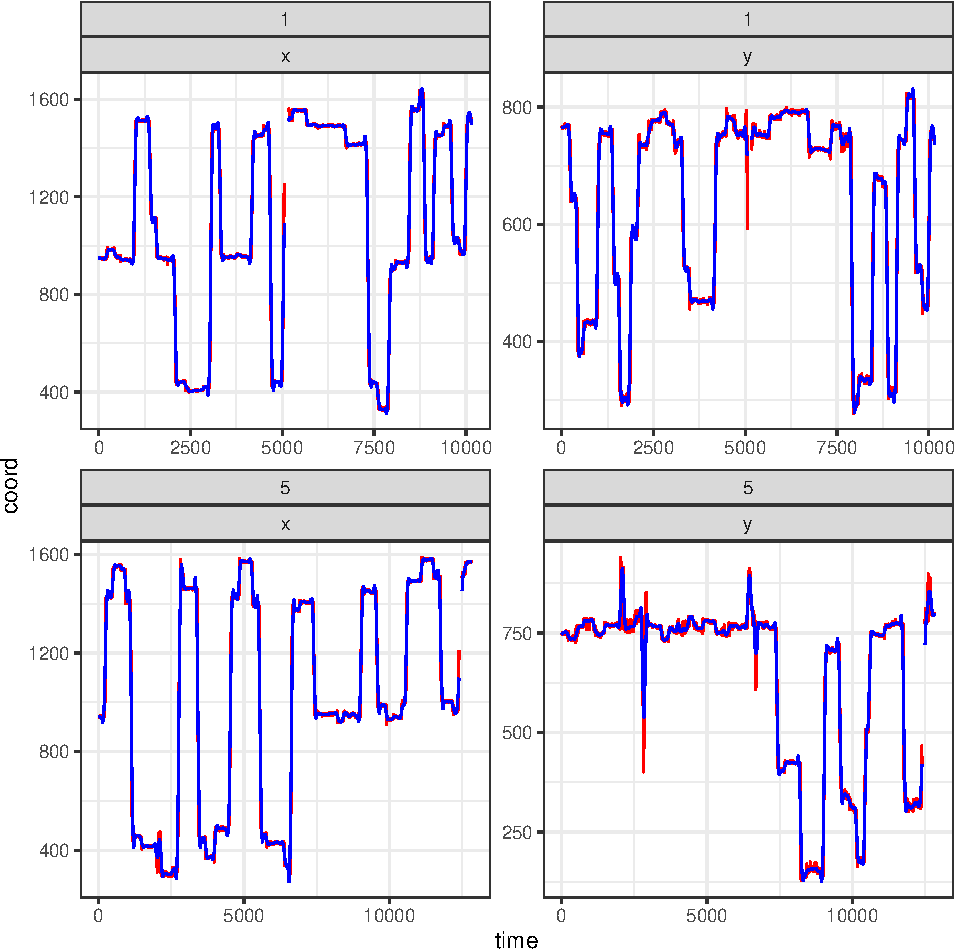
\includegraphics[keepaspectratio]{BRM_ms_files/figure-pdf/unnamed-chunk-6-1.pdf}}

\subsection{Fixations}\label{fixations}

Once the data has been repaired and smoothed, a core step in eye data
analysis is to identify fixations
(\citeproc{ref-salvucci2000identifying}{Salvucci \& Goldberg, 2000}),
defined as when the gaze stops in a specific location for a given amount
of time. When the eyes are moving between these fixations, they are
considered to be saccades. Subsequently, data can be split into these
two groups, fixations and saccades. In the eyetools package, there are
two fixation algorithms offered; the first algorithm,
\texttt{fixation\_dispersion()} employs a dispersion-based approach that
uses spatial and temporal data to determine fixations. By using a
maximum dispersion range, the algorithm looks for sufficient periods of
time that the eye gaze remains within this range and once this range is
exceed, this is termed as a fixation. The second algorithm,
\texttt{fixation\_VTI()} takes advantage of the idea that data is either
a fixation or a saccade and employs a velocity-threshold approach. It
identifies data where the eye is moving at a minimum velocity and
excludes this, before applying a dispersion check to ensure that the eye
does not drift during the fixation period. If the range is broken, a new
fixation is determined. Saccades must be of a given length to be
removed, otherwise they are considered as micro-saccades
{[}@CITATION\_NEEDED\_HERE?{]}.

Once fixations have been calculated, they can be used in conjunction
with Areas of Interest (AOIs) to determine the sequence in which the eye
enters and exits these areas, as well as the time spent in these
regions. When referring to AOIs, these often refer to the cues presented
and the outcome object. In our example, the two cues at the top of the
screen are the cues, and the outcome is at the bottom. We can define
these areas in a separate dataframe object by giving the centrepoint of
the AOI in x, y coordinates along with the width and height (if the AOIs
are rectangular) or just the radius (if circular).

In combination with the fixation data, the AOI information can be used
to determine the sequence of AOI entries using the \texttt{AOI\_seq()}
function. This fucntion checks whether a fixation is detected within an
AOI, and if not, it is dropped from the output, and then provides a list
of the sequence of AOI entries, along with start and end timestamps, and
the duration.

Time spent in AOIs can also be calculated from fixations or raw data
using the \texttt{AOI\_time()} function available. This calculates the
time spent in each AOI in each trial, based on the data type given, in
our case fixation data.

If choosing to work with the raw data, there is also the option of using
\texttt{AOI\_time\_binned()} which allows for the trials to be split
into bins of a given length, and the time spent in AOIs calculated as a
result.

\section{Analysing eye data}\label{analysing-eye-data}

@tom

\section{Discussion}\label{discussion}

In the present tutorial, we began by identifying the current gap in
available tools for working with eye data in open-science pipelines. We
then provided an overview of the general data collection process
required for eye tracking research, before detailing the conversion of
raw eye data into a useable eyetools format. We then covered the entire
processing pipeline using functions available in the eyetools package
that included the repairing and normalising the data, and the detection
of events such as fixations, saccades, and AOI entries.
@SOMETHING\_ON\_THE\_ANALYSIS\_GOES\_HERE.

From a practical perspective, this tutorial offers a step-by-step
walkthrough for handling eye data using R for open-science, reproducible
purposes. It provides a pipeline that can be relied upon by novices
looking to work with eye data, as well as offering new functions and
tools for experienced researchers. By enabling the processing and
analysis of data in a single R environment it also helps to speed up
data analysis.

\subsection{Advantages of Open-Source
Tools}\label{advantages-of-open-source-tools}

eyetools offers an open-source toolset that holds no hidden nor
proprietary functionality.

\section{Data Availability}\label{data-availability}

The data required for reproducing this tutorial is available at: @URL. A
condensed version of the dataset (starting with the
\texttt{combine\_eyes()} function) is a dataset in the eyetools package
called HCL.

\section{Code Availability}\label{code-availability}

The code used in this tutorial is available in the reproducible
manuscript file available at:

\section{References}\label{references}

\phantomsection\label{refs}
\begin{CSLReferences}{1}{0}
\bibitem[\citeproctext]{ref-duchowski2017eye}
Duchowski, A. T., \& Duchowski, A. T. (2017). \emph{Eye tracking
methodology: Theory and practice}. Springer.

\bibitem[\citeproctext]{ref-holmqvist2011eye}
Holmqvist, K., Nyström, M., Andersson, R., Dewhurst, R., Jarodzka, H.,
\& Van de Weijer, J. (2011). \emph{Eye tracking: A comprehensive guide
to methods and measures}. oup Oxford.

\bibitem[\citeproctext]{ref-orquin2019primer}
Orquin, J. L., \& Holmqvist, K. (2019). A primer on eye-tracking
methodology for behavioral science. In \emph{A handbook of process
tracing methods} (pp. 53--64). Routledge.

\bibitem[\citeproctext]{ref-rayner1998eye}
Rayner, K. (1998). Eye movements in reading and information processing:
20 years of research. \emph{Psychological Bulletin}, \emph{124}(3), 372.

\bibitem[\citeproctext]{ref-salvucci2000identifying}
Salvucci, D. D., \& Goldberg, J. H. (2000). Identifying fixations and
saccades in eye-tracking protocols. \emph{Proceedings of the 2000
Symposium on Eye Tracking Research \& Applications}, 71--78.

\end{CSLReferences}






\end{document}
